\section{Put it all together}

Sau khi kết hợp cả scheduling và memory, ta thực hiện make all và có kết qủa như các file log trong thư mục log/os*.txt


Dưới đây là giản đồ Gantt cho trường hợp trong log/all1.txt trong source code.

\textbf{Test 0:}

\vspace{0.5cm}

\begin{figure}[tph]
	\centering
	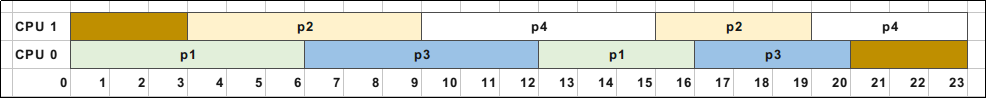
\includegraphics[width=13cm]{Images/all0.png}
	\vspace{0.5cm}
	\caption{Lược đồ Gantt CPU thực thi các processes cho make all}
	\label{fig:all0}
\end{figure}


\vspace{0.5cm}


\vspace{0.5cm}

\textbf{Test 1:}

\vspace{0.5cm}

\begin{figure}[tph]
	\centering
	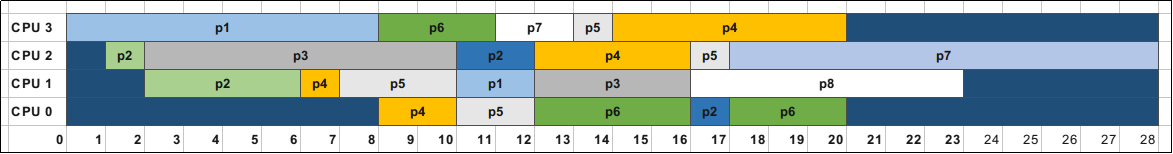
\includegraphics[width=15cm]{Images/all1.png}
	\vspace{0.5cm}
	\caption{Lược đồ Gantt CPU thực thi các processes cho make all}
	\label{fig:all1}
\end{figure}

\vspace{0.5cm}